%! suppress = UnresolvedReference


\chapter{\app 的需求分析}\label{ch:req}


\section{应用面向的用户群体}\label{sec:target-user}

本应用的目标用户是佩戴可穿戴动态心电信号监测设备的院外患者。由于心血管疾病的发病率随着年龄增长而增加\cite{Zhongguoxinxieguanjiankangyujibingbaogao20212022},有动态心电监测需求的患者也以中老年人为主。除了常规的功能性需求分析之外,本项目也结合用户群体的特征进行了额外的非功能性需求分析以及相关的设计和实现。


\section{应用的功能性需求分析}\label{sec:func-req}

本应用的用例图如图~\ref{fig:use-case} 所示。

\begin{figure}[ht]
    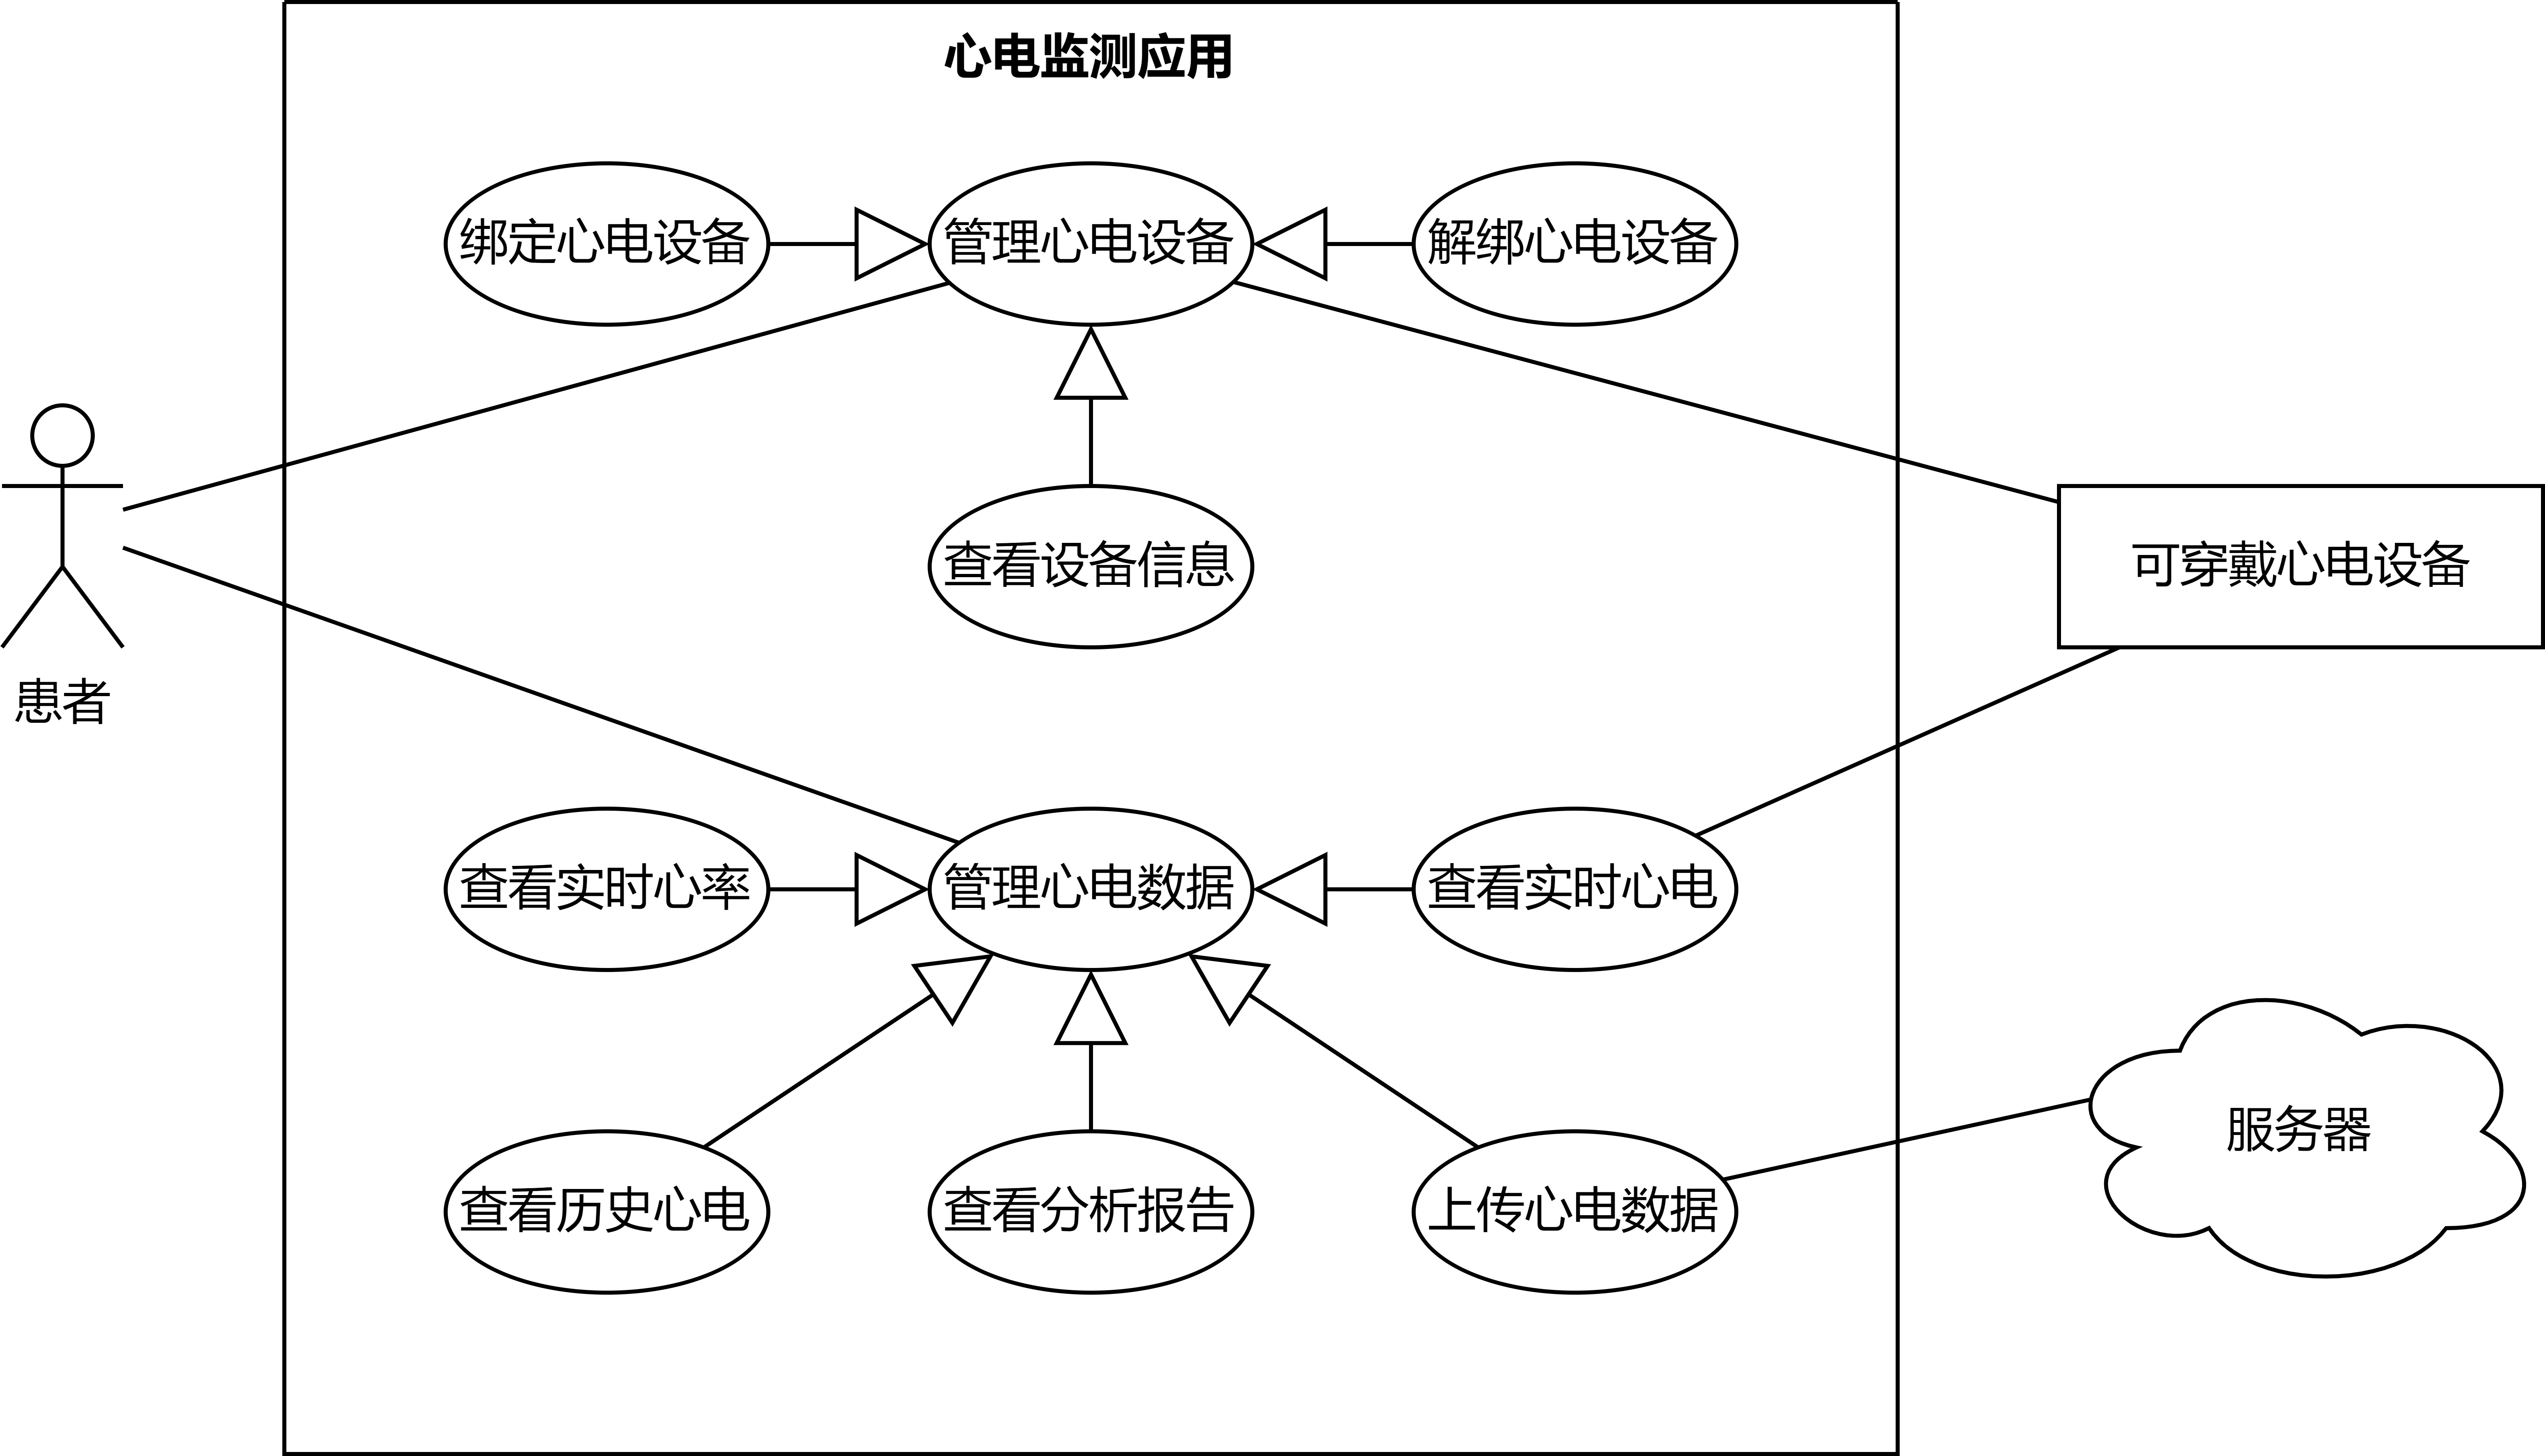
\includegraphics[width=\textwidth]{../assets/use-case.drawio}
    \bicaption{应用的用例图}{Use case diagram of the app}
    \label{fig:use-case}
\end{figure}

\subsection{管理心电设备的需求分析}\label{subsec:device-req}

\begin{itemize}
    \item[UC1] 用户可以通过应用程序绑定心电设备。
    \item[UC2] 用户可以通过应用程序断开心电设备的绑定。
    \item[UC3] 用户可以通过应用程序查看心电设备的名称。
    \item[UC4] 用户可以通过应用程序查看心电设备的型号。
    \item[UC5] 用户可以通过应用程序查看心电设备的连接状态。
    \item[UC6] 用户可以通过应用程序查看心电设备的信号质量。
    \item[UC7] 用户可以通过应用程序查看心电设备的电量。
\end{itemize}

\subsection{管理心电数据的需求分析}\label{subsec:ecg-req}

\begin{itemize}
    \item[UC8] 用户可以通过应用程序查看实时的心率数据。
    \item[UC9] 用户可以通过应用程序查看实时的心电图。
    \item[UC10] 用户可以通过应用程序查看历史的心电图。
    \item[UC11] 用户可以筛选要查看的历史心电图的时间。
    \item[UC12] 用户可以通过应用程序查看历史的心电分析报告。
    \item[UC13] 用户可以筛选要查看的历史心电分析报告的时间范围。
    \item[UC14] 用户可以通过应用程序上传心电数据到服务器。
\end{itemize}


\section{应用的非功能性需求分析}\label{sec:nonfunc-req}

\subsection{应用的易用性需求分析}\label{subsec:usability}

因为大部分中老年的用户没有丰富的移动设备使用经验,所以设计一个简单直观、易于使用的应用程序很重要。界面设计应避免使用复杂的元素,以尽量简洁清晰为目标。

此外,由于一般患者通常不会具备专业的医学知识,所以应用程序内应该尽可能地避免使用过于晦涩难懂的专业术语。同时,对于应用内无法避免使用的部分术语应该提供明显且易于理解的解释,以便用户理解其含义。

\subsection{应用的无障碍需求分析}\label{subsec:accessibility}

应用需要考虑到用户在视力等方面的障碍,尽可能地保证用户能够在不同的环境下使用应用程序。例如,应用程序应该提供对大字号、粗体字、高对比度、深浅主题等内容的支持。

\subsection{应用的性能需求分析}\label{subsec:performance}

由于动态心电监测的需要,本应用会长期驻留在系统后台运行。因此,应用程序的性能对于用户体验至关重要。应用程序应该尽可能地保持较低的内存占用和较低的电量消耗,以保证用户的使用体验。

\subsection{应用的兼容性需求分析}\label{subsec:compatibility}

应用程序需要能够在各种主流移动设备上运行。这包括对于Android和iOS两大移动操作系统的支持,以及对于各种型号的移动设备的支持。在应用的设计与实现中,需要充分考虑到不同环境可以为应用提供的可用功能有所差别,以保证应用程序在不同环境下的兼容性。


\section{项目的可行性分析}\label{sec:feasibility}

\todo{项目是否可行?为什么?(事实证明是可行的,但还是得站在项目开始前的视角分析一下。)}
